\documentclass[a4paper,10pt,ngerman]{scrartcl}
\usepackage{babel}
\usepackage{hyperref}
\usepackage[T1]{fontenc}
\usepackage[utf8x]{inputenc}
\usepackage[a4paper,margin=2.5cm,footskip=0.5cm]{geometry}

\newcommand{\Aufgabe}{Aufgabe 3: Hex-Max} % Aufgabennummer und Aufgabennamen angeben
\newcommand{\TeamId}{00730}                       % Team-ID aus dem PMS angeben
\newcommand{\TeamName}{SilverBean}                 % Team-Namen angeben
\newcommand{\Namen}{Philip Gilde}           % Namen der Bearbeiter/-innen dieser Aufgabe angeben
 
\usepackage{scrlayer-scrpage, lastpage}
\setkomafont{pageheadfoot}{\large\textrm}
\lohead{\Aufgabe}
\rohead{Team-ID: \TeamId}
\cfoot*{\thepage{}/\pageref{LastPage}}

% Position des Titels
\usepackage{titling}
\setlength{\droptitle}{-1.0cm}

% Für mathematische Befehle und Symbole
\usepackage{amsmath}
\usepackage{mathtools}
\DeclareMathOperator*{\argmax}{arg\,max}
\usepackage{amssymb}

% Für Bilder
\usepackage{graphicx}
\graphicspath{ {./bilder/}}
% Für Algorithmen
\usepackage{algpseudocode}

% Für Quelltext
\usepackage{listings}
\lstset{literate=%
  {Ö}{{\"O}}1
  {Ä}{{\"A}}1
  {Ü}{{\"U}}1
  {ß}{{\ss}}1
  {ü}{{\"u}}1
  {ä}{{\"a}}1
  {ö}{{\"o}}1
}
\usepackage{wrapfig}
\usepackage{color}
\definecolor{mygreen}{rgb}{0,0.6,0}
\definecolor{mygray}{rgb}{0.5,0.5,0.5}
\definecolor{mymauve}{rgb}{0.58,0,0.82}
\lstset{
  keywordstyle=\color{blue},commentstyle=\color{mygreen},
  stringstyle=\color{mymauve},rulecolor=\color{black},
  basicstyle=\footnotesize\ttfamily,numberstyle=\tiny\color{mygray},
  captionpos=b, % sets the caption-position to bottom
  keepspaces=true, % keeps spaces in text
  numbers=left, numbersep=5pt, showspaces=false,showstringspaces=true,
  showtabs=false, stepnumber=2, tabsize=2, title=\lstname
}
\lstdefinelanguage{JavaScript}{ % JavaScript ist als einzige Sprache noch nicht vordefiniert
  keywords={break, case, catch, continue, debugger, default, delete, do, else, finally, for, function, if, in, instanceof, new, return, switch, this, throw, try, typeof, var, void, while, with},
  morecomment=[l]{//},
  morecomment=[s]{/*}{*/},
  morestring=[b]',
  morestring=[b]",
  sensitive=true
}
\usepackage{csquotes}
\newcommand\mdoubleplus{\mathbin{+\mkern-10mu+}}
% Diese beiden Pakete müssen zuletzt geladen werden
%\usepackage{hyperref} % Anklickbare Links im Dokument
\usepackage{cleveref}

% Daten für die Titelseite
\title{\textbf{\Huge\Aufgabe}}
\author{\LARGE Team-ID: \LARGE \TeamId \\\\
	    \LARGE Bearbeiter dieser Aufgabe: \\ 
	    \LARGE \Namen\\\\}
\date{\LARGE\today}

\begin{document}

\maketitle
\tableofcontents

\vspace{0.5cm}



\section{Lösungsidee}

Zunächst sollten die Dynamiken einer Transformation, also einer Folge von Verschiebungen, bei der aus einer Hexzahl eine andere wird, betrachtet werden, unabhängig davon, wie groß die sich ergebende Zahl ist. Im Folgenden markiert das Apostroph $'$ eine Zahl nach der Transformation. Eine einzelne Ziffer lässt sich als Liste von 7 booleschen Werte darstellen: Für jedes Segment ein Wert, der aussagt, ob ein Stäbchen vorhanden ist oder nicht. Die Reihenfolge wird folgendermaßen definiert: \\
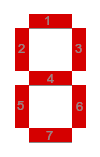
\includegraphics[scale=4]{ziffereinzel} \\
 Wenn man nun eine Ziffer $Z$ in eine andere Ziffer $Z'$ umlegen möchte, ist das nur möglich, wenn die Ausgangs- und Zielziffer gleich viele Stäbchen haben, also gleich viele Werte wahr sind. Das ist die erste Bedingung ($C(X)$ ist die Anzahl wahrer Werte in der Liste $X$):
\begin{align}
&& C(Z) &= C(Z') && |-C(Z') \\
\leftrightarrow && C(Z) - C(Z') &= 0 && \\
&& D(Z, Z') &\coloneqq C(Z) - C(Z') && \\
&& D(Z, Z') &= 0 && \\
\end{align}
Die Anzahl der verschobenen Stäbchen lässt sich finden, in dem man für jedes Stäbchen von $Z$ prüft, ob dieses auch bei $Z'$ vorhanden ist. Ist dies nicht der Fall, muss dieses Stäbchen umgelegt werden. Die Anzahl $R(Z, Z')$ an zu verschiebenden Stäbchen für die beiden Ziffern $Z$ und $Z'$ darf nicht größer als $m$ sein. Das ist die zweite Bedingung: 
\begin{align}
R(Z, Z') &\coloneqq C(Z \land \neg Z') \\
R(Z, Z')&\leq m
\end{align}
Eine mehrstellige Zahl setzt sich aus den $l$ Ziffern $Z_0, Z_1, Z_2, ... \,Z_{l-1}, Z_l$ vor der Transformation beziehungsweise $Z_0', Z_1', Z_2', ... \,Z_{l-1}', Z_l'$ nach der Transformation zusammen.
Die Konkatenation dieser Ziffern wird im folgenden als $Q$ beziehungsweise $Q'$ bezeichnet. Die beiden Bedingungen gelten genauso für $Q$ und $Q'$ anstelle von $Z$ und $Z'$. \\
Die Anzahl an wahren Werten einer Konkatenation ist gleich der Summe der Anzahlen an wahren Werten der konkatenierten Listen. Wenn beispielsweise eine Liste 5 wahre Werte enthält und eine andere 3, wird die Konkatenation dieser 8 wahre Werte enthalten ($A\circ V$ steht für die Konkatenation der Listen $A$ und $B$):
\begin{align}
C(A \circ B) = C(A) + C(B)
\end{align}
Wenn also gilt:
\begin{align}
C(Q) &= C(Q')
\end{align}
Dann gilt auch, weil $Q$ ja die Konkatenation von $Z$ ist:
\begin{align}
&&\sum_{n=0}^l C(Z_n) &= \sum_{n=0}^l C(Z'_n)&& |-\sum_n^l C(Z'_n) \\
\leftrightarrow && \sum_{n=0}^l (C(Z_n) - C(Z_n')) &= 0 && \\
&& \sum_{n=0}^l D(Z_n, Z_n') &= 0 
\end{align}
Eine einzelne Ziffer $Z_k$ lässt sich abkapseln:
\begin{align}
&& \sum_{n=0}^l D(Z_n, Z_n') &= 0 && |-D(Z_k, Z_k')) \\
\leftrightarrow && \sum_{n=0|n \neq k}^l D(Z_n, Z_n') &= -D(Z_k, Z_k') &&
\end{align}
So lässt sich die erste Bedingung zu einer Ziffer hin umstellen. Dadurch kann man eine einzelne Ziffer transformieren und erhält daraus eine Bedingung für die restlichen Ziffern.\\
Bei der zweiten Bedingung verhält es sich genauso:
\begin{align}
&&R(Q, Q') &\leq m \\
&&\sum_{n=0}^l R(Z_n, Z_n') &\leq m & |-R(Z_k, Z_k') \\
\leftrightarrow && \sum_{n=0|n \neq k}^l R(Z_n, Z_n') &\leq m -R(Z_k, Z_k')
\end{align}

Auf diese Weise lässt sich eine rekursive Suche nach der höchstmöglichen Zahl, die die Bedingungen erfüllt, konstruieren. Dabei wird zuerst die ganz links stehende Ziffer auf den höchsten Wert gesetzt und für die restlichen Ziffern eine möglichst hohe Zahl gesucht, mit der die Bedingungen erfüllt wird. Es wird also mit den restlichen Ziffern genauso verfahren bis zur letzten Ziffer. Die von links erste Ziffer $Z_0'$ wird auf den höchstmöglichen Wert F gesetzt. Für die restlichen Ziffern gilt dann 
\begin{align}
\sum_{n \neq 0}^l D(Z_n, Z_n') &= -D(Z_0, Z_0') \\
\sum_{n \neq 0}^l R(Z_n, Z_n') &\leq m - R(Z_0, Z_0') 
\end{align}
Wenn bei der zweiten Bedingung $m-R(Z_0, Z_0')$ kleiner als 0 ist, würden durch die Transformation mehr Stäbchen bewegt als erlaubt ist, weil daraus folgen würde, dass $m<R(Z_0, Z_0')$. Es wird dann mit dem nächst kleineren Wert für die Stelle weiter gesucht. Wenn $m-R(Z_0, Z_0')$ gleich $0$ ist, wurden schon so viele Stäbchen weggenommen, wie erlaubt ist. Wenn die Bedingung (18) so schon erfüllt ist, wurden auch so viele Stäbchen an anderen Stellen hingelegt. Wenn nicht, müssen diese Stäbchen noch weiter hinten hingelegt werden. Im ersten Fall wird die Suche beendet, da die so gebildete Zahl die höchstmögliche ist. Sie ist die höchstmögliche, weil die signifikantesten Stellen auf die höchstmöglichen Werte gesetzt wurden und die restlichen nicht mehr änderbar sind. Im zweiten wird für die restlichen Ziffern mit den veränderten Bedingungen (18) und (19) weiter gesucht.\\
Wenn $m-R(Z_0, Z_0')$ größer als Null ist, wird mit den restlichen Ziffern der gleiche Prozess durchgeführt, um die höchstmögliche Zahl zu finden. Sie muss die Bedingungen (18) und (19) erfüllen.\\
Wenn sich mit den restlichen Ziffern die Bedingung erfüllende Zahlen finden lassen, ist die höchste dieser in Verbindung mit $Z_0'$ die höchstmögliche Zahl. Wenn nicht, wird die erste Ziffer um 1 reduziert und dasselbe wiederholt. Es ist nicht möglich, dass die Zahl kleiner wird, als sie vorher war, weil eine Transformation einer Zahl zu sich selbst zwangsläufig beide Kriterien erfüllt. \\
Das Verfahren lässt sich mit einem Suchbaum modellieren:\\
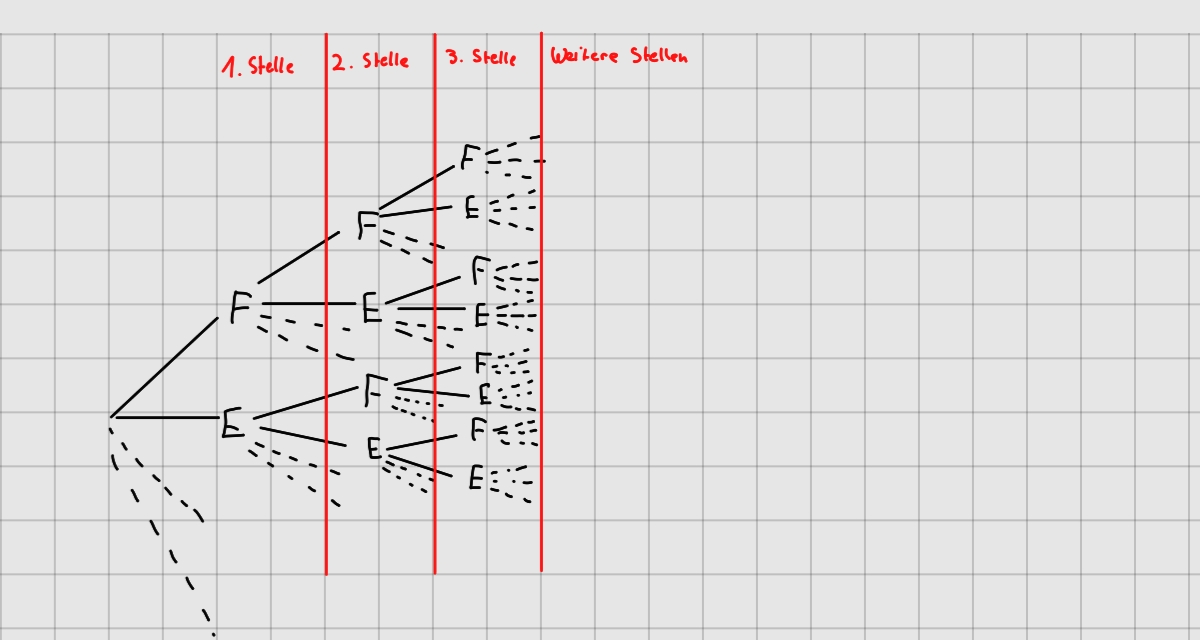
\includegraphics[width=\textwidth]{suchbaum1}\\
Für die erste Stelle gibt es 16 Äste für jede mögliche Ziffer. In der Zeichnung wurden nur die obersten 2 dargestellt, der Rest soll mit den gestrichelten Linien angedeutet werden. Von jedem dieser 16 Äste gehen jeweils 16 weitere Äste ab, für jede mögliche zweite Ziffer (nicht eingezeichnete Äste sind wieder durch gestrichelte Linien angedeutet). So geht es immer weiter bis zur letzten Ziffer. Das Verfahren geht dabei erst den obersten Ast entlang, dann den (am Ende) zweithöchsten und so weiter. Dabei kann die Suche abgebrochen werden, sobald eine passende Ziffer gefunden wurde, weil ja alle weiteren Ziffern kleiner sind beziehungsweise alle größeren schon durchsucht wurden, ohne die Bedingungen zu erfüllen. \\
Das Verfahren soll an der Beispieleingabe \lstinline|D24| mit $m=3$ illustriert werden. Die Zahl sieht im 7-Segment-Display so aus: \\
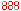
\includegraphics[width=0.5\textwidth]{bild1}\\
Es wird die erste Ziffer von D auf F gesetzt. Dabei werden 3 Stäbchen von ihrer aktuellen Position weggenommen: $R(Z, Z')=3$. Die Differenz an Stäbchen nach der Transformation liegt bei -1, es bleibt also ein Stäbchen übrig. Für die beiden restlichen Ziffern dürfen also keine Stäbchen von ihrer Position vor der Transformation weggenommen werden. Die Differenz muss dagegen bei 1 liegen, damit die Summe $0$ ist. Es muss also ein Stäbchen aufgebraucht werden, damit das bei der ersten Ziffer übrig gebliebene einen Platz findet. Mit diesen beiden Bedingungen wird nun also die größtmögliche Transformation der übrigen Ziffern \lstinline|24| mit dem selben Verfahren gesucht. Die erste Ziffer wird auf F gesetzt, dabei werden allerdings Stäbchen von ihrer Ursprungsposition weggenommen, womit $R(Z, Z') > 3$ wäre, es wird also bei der nächst-kleineren Ziffer weiter gesucht. Bei allen kleineren Ziffern bis zur 8 werden Stäbchen von ihrer Position weggenommen. Bei der 8 werden zwei Stäbchen zugelegt, die Differenz für die einzelne Ziffer ist also 2, die gesamte Differenz beträgt $-1 + 2 = 1$. Damit die Anzahl der Stäbchen sich nicht ändert, muss bei der letzten Ziffer die Differenz -1 sein, es muss also ein Stäbchen weggenommen werden. Da aber kein Stäbchen mehr weggenommen werden darf (sonst wäre $R(Z, Z') > 3$), lässt sich nach Durchprobieren aller keine letzte Ziffer finden, welche die Bedingungen erfüllt. Es wurde keine Lösung gefunden, also wird bei der Ziffer an der vorherigen Stelle weiter probiert. Die nächste Zahl, bei der kein Stäbchen weggenommen wird, ist die 2. Für die zwei ist die Differenz 0, es muss ja nichts umgelegt werden. Bei der letzten Ziffer muss die Differenz 1 sein, also ein Stäbchen hinzu gelegt werden. Es darf aber kein Stäbchen umgelegt werden, da dann $R(Z, Z') > 3$ wäre. Nur durch hinlegen eines Stäbchens lässt sich aus der 4 keine andere Ziffer bilden, es muss also bei der Stelle davor weiter gesucht werden. Dort gibt es keine weiteren Ziffern, zu denen transformiert werden kann, ohne ein Stäbchen irgendwo wegzunehmen. Weil keine Lösung gefunden wurde, wird also bei der ersten Ziffer weiter gesucht. Diese wird auf den nächst-kleineren Wert E gesetzt. Bei dieser Umwandlung werden nur zwei der ursprünglichen Stäbchen weggenommen. Die Differenz der Stäbchenzahlen ist 0. Bei den restlichen Ziffern darf also ein Stäbchen von seiner ursprünglichen Position weggenommen werden, während die Differenz der Stäbchenzahlen 0 sein muss. Wie vorher wird nun die größtmögliche Zahl für die restlichen Ziffern gesucht. Die Ziffer an zweiter Stelle wird auf von 2 auf F gesetzt. Dabei wird allerdings mehr als 1 Stäbchen von seiner ursprünglichen Position entfernt, die Bedingungen sind nicht erfüllt. Bei der Transformation von 4 zu E hingegen muss nur ein Stäbchen von seiner ursprünglichen Position entfernt werden. Damit wurden insgesamt genau $3=m$ Stäbchen von ihrer ursprünglichen Position entfernt. Die Gesamtdifferenz beträgt 0, es können also bei der letzten Ziffer keine Stäbchen zugelegt werden. Somit ist die Lösung \lstinline|EE4| gefunden, welche laut Aufgabenblatt richtig ist. \\
Um die Anzahl von zu durchsuchenden Zahlenfolgen zu reduzieren, können weitere Bedingungen für die Fortsetzung der Suche mit den restlichen Ziffern eingeführt werden. Eine solche Bedingung ist, dass der Überschuss an weggenommenen beziehungsweise hingelegten Stäbchen mit den restlichen Ziffern ausgeglichen werden kann. Wenn die ursprüngliche Zahl beispielsweise 88888 ist, mit $m=10$, lässt sich keine größere Zahl finden, die durch Umlegung erreicht werden kann, weil jede andere Zahl weniger Stäbchen hätte und somit bei der Transformation Stäbchen übrig blieben. Damit nicht jede Zahlenfolge von FFFFF bis 88888 durchprobiert werden muss, um das zu "bemerken", wird nach jeder Transformation einer einzelnen Ziffer geprüft, ob die Differenz der Stäbchenzahlen der bisherigen Transformation $D$ durch Transformation der restlichen Ziffern kompensiert werden könnte. Dafür werden mit den restlichen Ziffern die beiden Differenzen der Stäbchenzahlen $D_{min}$ bei einer Transformation jeder Ziffer zu einer 8, und $D_{max}$ bei Transformation jeder Ziffer zu einer 1, berechnet. 8 hat mit 7 Stäbchen die größte Zahl an Stäbchen und 1 mit 2 die kleinste.\\ Wenn $D > -D_{min}$, wurden mehr Stäbchen von den transformierten Ziffern weggenommen, als bei den restlichen Ziffern hingelegt werden könnten. Wenn $D < -D_{max}$, würden für die transformierten Ziffern mehr zusätzliche Stäbchen benötigt, als von den restlichen Ziffern weggenommen werden könnten. Ein Beispiel für den ersten Fall wäre die Transformation von \lstinline|111| zu \lstinline|F11|. Ein Beispiel für den zweiten Fall ist das obige mit 88888 als ursprüngliche Zahl. \\
Eine weitere Möglichkeit, die Anzahl der zu durchsuchenden Zahlenfolgen zu reduzieren, ist zu prüfen, ob $R(Z', Z) \leq m$ und die Suche nur zu vertiefen, wenn es der Fall ist. Durch das Tauschen der Reihenfolge wird hier nicht gezählt, wie viele Stäbchen von ihrer ursprünglichen Position weggenommen wurden, sondern wie viele Stäbchen in vorherigen Lücken liegen. Bei einer gültigen Transformation haben beide den gleichen Wert, weil jedes weggenommene Stäbchen an einer anderen Stelle hingelegt wird, wo vorher keines war. Da die Transformationen bei der Suche allerdings nicht vollständig sind, kann es sein, dass einer der beiden Werte noch kleiner gleich $m$ ist, während der andere schon größer ist. \\
Weiterhin kann geprüft werden, ob die Differenz der Stäbchenzahlen noch ausgeglichen werden kann, ohne das $m$ dabei überschritten wird. Wenn also beispielsweise bei einer Teiltransformation, die noch vertieft werden muss, $m=10$, $R(Z, Z')=6$ und $D=-5$, dann kann die Differenz nicht mehr kompensiert werden, weil bei den restlichen Ziffern 5 Stäbchen übrig bleiben müssen, aber nicht nur noch 4 Stäbchen weggenommen werden dürfen, damit $R(Z, Z') \leq m$ ist. Wenn also $-D>m-R(Z, Z')$ gilt, kann die Differenz nicht kompensiert werden und es wird nicht vertieft. Umgekehrt darf nicht $D>m-R(Z, Z')$ sein, dann sind schon mehr Stäbchen übrig geblieben, als noch hingelegt werden dürfen. \\
Zuletzt muss bei einer Vertiefung der Suche diese nicht immer nochmal durchgeführt werden. Wenn beispielsweise die erste Ziffer eine 8 ist, kann es sein, dass diese bei der Suche irgendwann in ein E transformiert wird. Dabei werden zwei Stäbchen von ihrer Ursprungsposition weggenommen und bleiben übrig. Wenn die Vertiefung der Suche ergibt, dass mit dieser Transformation keine passende Anordnung für die restlichen Ziffern gefunden werden kann. Es wird also mit Transformation zu D weitergesucht. Bei dieser werden, genau wie beim E, zwei Stäbchen weggenommen und bleiben übrig. Die Bedingungen für die restlichen Zahlen sind also gleich und es muss nicht nochmal die ganze Suche durchgeführt werden, um zu wissen, dass die Bedingungen nicht erfüllt werden kann. \\
Wenn $Z'$ gefunden ist, muss die Reihenfolge der Umlegungen ermittelt werden. Dabei muss laut Aufgabenstellung zu jedem Zeitpunkt bei jeder Ziffer mindestens ein Stäbchen liegen. Dafür wird eine zunächst leere Liste von Umlegungen $L$ und der Zwischenzustand $Z^*$ eingeführt, welcher anfangs gleich der Ausgangszahl ist. Nun wird für jedes Segment $Z_{j,k}^*$ von $Z^*$ geprüft ($j$ ist die Zahl der Ziffer und $k$ des Segments in dieser), dort ein Stäbchen liegt, aber nicht bei $Z_{j,k}'$, also $Z^*_{j,k} \land \neg Z_{j,k}'$. Wenn ja, muss dieses Stäbchen verlegt werden. Wenn das Stäbchen das einzige Stäbchen seiner Ziffer ist, wird bei der nächsten Ziffer weitergemacht und das Stäbchen wird später verlegt. Wenn nicht, wird bei $Z'$ nach einem Segment gesucht, bei dem ein Stäbchen liegt, an dessen Stelle aber bei $Z^*$ noch keines liegt. Es werden also $q,r$ gesucht, für die gilt $Z'_{q,r} \land \neg Z^*_{q,r}$. Diese Verschiebung des Stäbchens bei $j,k$ nach $q,r$ wird in $Z^*$ durchgeführt und an das Ende von $L$ gehangen. $Z_{j,k}^*$ wird weiter durch das veränderte $Z^*$ iteriert. Wenn das letzte Segment erreicht ist, wird wieder von vorne begonnen. Es wird so lange iteriert, bis $Z^*=Z'$. Dann wurden alle Schritte gefunden.
\section{Umsetzung}
Die Aufgabe wurde in Python implementiert. Dabei wurde die Klasse \lstinline|HashableArray| eingeführt, die eine oder mehrere Ziffern repräsentiert. Die Klasse ermöglicht die notwendigen elementweisen Operationen \textit{und} und \textit{nicht}, so wie das Zählen der Stäbchen. Diese Operationen werden auch von NumPy-Arrays unterstützt, allerdings sind diese veränderbar und können deshalb nicht gehasht und somit als Schlüssel in einem \lstinline|dict| verwendet werden. Das ist notwendig, weil der zur Python-Standardbibliothek gehörende Dekorator \lstinline|functools.lru_cache| sonst nicht verwendet werden kann. Dieser Dekorator speichert die Ergebnisse von Funktionen, damit diese bei gleichen Argumenten nicht nochmal ihre ganze Laufzeit brauchen, sondern das Ergebnis (in der Regel) innerhalb von $\mathcal{O}(1)$ abgerufen werden kann. Damit wird die in der Lösungsidee beschriebene nicht-Durchführung der Vertiefung der Suche bei gleichen Bedingungen implementiert. Weil das Verfahren rekursiv implementiert wurde, musste die Begrenzung der Rekursionstiefe von Python mit \lstinline|sys.setrecursionlimit(3000)| auf 3000 erhöht werden. Mit dieser Tiefe konnte selbst die Beispieleingabe auf der BwInf-Webseite mit 1000 Ziffern gelöst werden, für höhere Werte wurde das Programm nicht getestet. \\
Wenn das Programm aufgerufen wird, muss erst der Pfad zur Datei mit der Eingabe angegeben werden, und dann, ob die einzelnen Schritte ausgegeben werden sollen.
\section{Laufzeit}
Es wenn die eingegebene Zahl $Z$ die Länge $n$ hat, müssen höchstens $16^n-Z$ verschiedene Zahlen durchprobiert werden. Eine wirkliche Abschätzung der Laufzeit ist schwierig, weil der Einfluss der Bedingungen für die Vertiefung der Suche hochgradig abhängig von der eingegeben Zahl ist. Der Speicherbedarf wächst linear zu $n$, da immer nur die aktuelle Teiltransformation, welche aus höchstens $n$ Ziffern besteht, gespeichert werden muss. Beim Speichern der Ergebnisse von Vertiefungen der Suche kann der Speicherbedarf theoretisch schnell ansteigen, allerdings wurde die Größe des \lstinline|functools.lru_cache|, welcher dies implementiert, begrenzt. Bei der längsten Beispieleingabe lag der maximale Arbeitsspeicherbedarf bei circa 58 MB. Diesen Wert erachte ich als akzeptabel, weil die meisten aktuellen Computer wenigstens 1 GB Arbeitsspeicher für Programme zur Verfügung stellen.
\section{Beispiele}

\section{Quellcode}
\lstinputlisting[language=python]{hexmax.py}

\end{document}
